\documentclass{article}
\usepackage{graphicx}
\graphicspath{ {./img/} }
\usepackage{amsmath}
\usepackage{amsfonts}
\usepackage{amssymb}
\usepackage[left=1.5cm, right=1.5cm, top=1.5cm, bottom=1.5cm]{geometry}

\DeclareMathOperator{\Span}{span}
\newcommand{\sa}{\Span(\mathbb{A})}
\newcommand{\V}{\mathbb{V} (\mathbb{K})}
\newcommand{\s}[2]{#1_1, #1_2, \ldots, #1_{#2}}
\newcommand{\Vx}[1]{\mathbb{V}_#1 (\mathbb{K})}
\newcommand{\ah}{\alpha}
\newcommand{\bh}{\beta}
\newcommand{\ch}{\gamma}


\title{Algebra Lineare e Geometria Analitica}
\author{Andrea Bellu}
\date{2023/2024}

\begin{document}

\maketitle

\tableofcontents

\section{Spazi Vettoriali}
Siano $K$ un campo e $V$ un insieme. Si dice che $V$ è uno spazio vettoriale
sul campo $K$, se sono definite due operazioni: un’operazione interna binaria
su $V$, detta somma, $+: V \times V \mathbb{R}\rightarrow V$ e un’operazione
esterna, detta prodotto esterno o prodotto per scalari, $\bullet : K \times V \mathbb{R}\rightarrow V$, tali che:

\begin{enumerate}
    \item $(V, +)$ sia un gruppo abeliano;
    \item il prodotto esterno $\bullet$ soddisfi le seguenti proprietà:
          \begin{enumerate}
              \item $(h\cdot k)\bullet \bar{v} = h\bullet(h\bullet \bar{v}) \ \ \ \forall h,k \in K \ \ \ \text{e} \ \ \ \forall \bar{v} \in V$
              \item $(h+ k)\bullet \bar{v} = h\bullet \bar{v}+k\bullet \bar{v} \ \ \ \forall h,k \in K \ \ \ \text{e} \ \ \ \forall \bar{v} \in V$
              \item $h\bullet(\bar{v}+\bar{w}) = h\bullet\bar{v}+h\bullet\bar{w} \ \ \ \forall h,k \in K \ \ \ \text{e} \ \ \ \forall \bar{v} \in V$
              \item $1\bullet \bar{v} = \bar{v} \ \ \ \forall \bar{v} \in V$ ove 1 è l’unità del campo $K$
          \end{enumerate}
\end{enumerate}

$V(K) = (V, K, +:V\times V\mathbb{R}\rightarrow V, \bullet:K\times V\mathbb{R}\rightarrow V) \implies$ struttura algebrica

Gli elementi dell’insieme $V$ sono detti \textbf{vettori} gli elementi del
campo $K$ sono detti \textbf{scalari}.

\subsubsection{Nota bene}
Sia $\mathbb K$ un campo, indichiamo con $\mathbb K_{[x]}=\{a_0+a_1x+\cdots \ | \ a_i\in\mathbb K\}$ l'insieme di tutti i polinomi in $x$ a coefficienti in $\mathbb K$.

\subsection{Vettori}
I vettori sono segmenti orientati con \textbf{verso, direzione e lunghezza}.
\begin{figure}[ht]
    \centering
    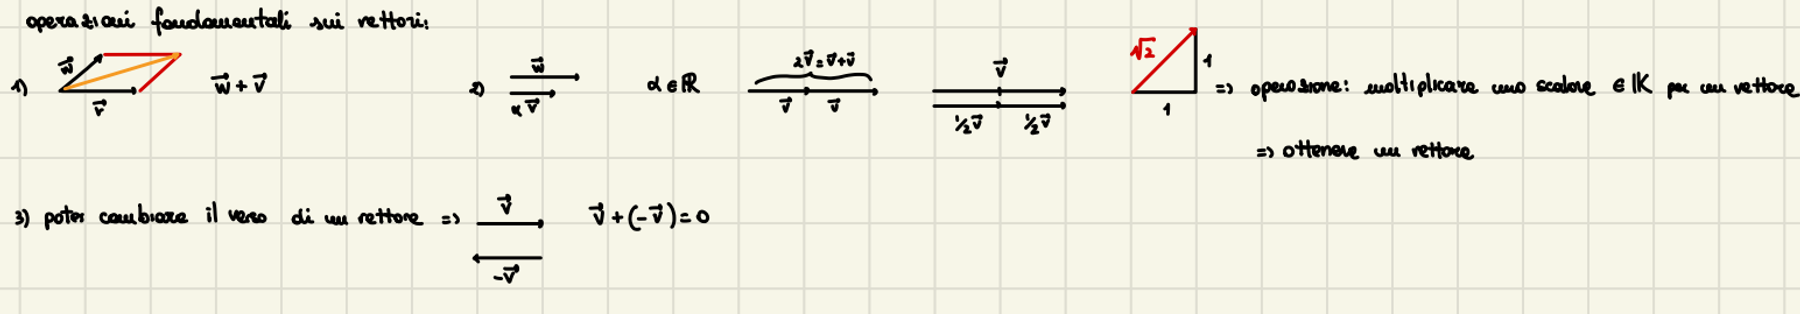
\includegraphics[width=1\linewidth]{image.png}
    \caption{Vettori}\label{fig:enter-label}
\end{figure}

\subsubsection{Esercizio}
Sia $\mathbb{R}^2$ con le operazioni di somma componente per componente
$\implies$ $(a, b) + (c, d) = (a+c, b+d)$ e prodotto per scalare campo per
campo $\alpha(a,b) = (\alpha a, \alpha b)$ è uno spazio vettoriale reale.

\begin{enumerate}
    \item Far vedere che $(\mathbb{R}^2,+)$ è un gruppo abeliano:
          \begin{enumerate}
              \item $\forall a,b \in \mathbb{R}^2 : (a,b)+(0,0) = (a+0, b+0) = (a,b) = (0+a, 0+b) = (0,0)+(a,b)$
              \item $\forall a,b \in \mathbb{R}^2 \ \ \exists \ (-a, -b) \in \mathbb{R}^2:(a,b)+(-a, -b) = (a-a, b-b) = (0,0) = (-a+a, -b+b) = (-a, -b)+(a,b)$
              \item  $\forall(a,b),(c,d),(e,f) \in \mathbb{R}^2 : (a,b)+ ((c,d)+(e,f)) = (a,b) + (c+e, d+f) = (a+ (c+e), b+ (d+f)) = ((a+c)+e, (b+d)+f) = (a+c, b+d)+(e,f)=((a,b)+(c,d))+(e,f)$
              \item  $(a,b)+(c,d)=(a+c, b+d)=(c+a,d+b)=(c,d)+(a,b)$
          \end{enumerate}
\end{enumerate}

Abbiamo verificato che $(\mathbb{R}^2,+)$ è un gruppo abeliano.

NB\@:  abbiamo usato solamente che $\mathbb{R}$ è un campo $\implies$ abbiamo
usato solo le proprietà della somma
\begin{enumerate}
    \item Ora dobbiamo verificare che il prodotto esterno soddisfi le proprietà dello
          spazio vettoriale:
          \begin{enumerate}
              \item $\forall a,b,c \in \mathbb{R}^2 : 1\cdot(a,b)=(1\cdot a, 1\cdot b) = (a,b)$ $\implies$ elemento neutro
              \item $\alpha,\beta \in \mathbb{R}^2 = (\alpha\beta)\cdot(a,b)=((\alpha\beta)a, (\alpha\beta)b) = (\alpha(\beta a, \alpha(\beta b)) = \alpha(\beta a, \beta b) = \alpha(\beta \cdot(a,b))$ $\implies$ pseudo associativa
              \item $\forall \alpha,\beta\in\mathbb{R} \ \ \ (a,b) \in \mathbb{R}^2 : (\alpha+\beta)(a,b) = ((\alpha+\beta)a, (\alpha+\beta)b)=(\alpha a+\beta a, \alpha b + \beta b) = (\alpha a, \alpha b)+(\beta a, \beta b) = \alpha(a,b) + \beta(a,b)$ $\implies$ pseudo distributiva
              \item $\forall \alpha \in \mathbb{R} (a,b) ,(c,d) \in \mathbb{R}^2 : \alpha((a,b)+(c,d)) = \alpha(a+c,b+d)=(\alpha a, \alpha c, \alpha b, \alpha d)=(\alpha a, \alpha b) + (\alpha c, \alpha d) = \alpha(a,b)+\alpha(c,d)$
          \end{enumerate}

\end{enumerate}

\subsection{Combinazione Lineare}
Siano $\bar{v_1}\dots.\bar{v_k}\in V(\mathbb{K})$ vettori, $\alpha_1, \alpha_n$
scalari, si dice combinazione lineare di $(\bar{v_1}\dots\bar{v_k})$ con
$\alpha_1,\alpha_k$ il vettore $\alpha_1\bar{v_1}+\cdots+\alpha_n\bar{v_k}$.

\subsection{Applicazione Lineare}
Siano $V(\mathbb{K}) \ \ \text{e}\ \ W(\mathbb{K})$ due spazi vettoriali su
$\mathbb{K}$. Si dice applicazione lineare da $V(\mathbb{K}) \ \ \text{in} \ \
    W(\mathbb{K})$ una funzione $f:V\rightarrow W$ tale che

\[
    \forall \bar{v}, \bar{w}\in W, \forall\alpha,\beta\in\mathbb{K} \ \ \ f(\alpha\bar{w}+\beta\bar{v})=\alpha f(\bar{w})+\beta f(\bar{v})
\]
Un’applicazione lineare è una funzione che manda combinazioni lineari di vettori in combinazioni lineari con i medesimi coefficienti.
Se $V(\mathbb{K})$ è spazio vettoriale e $f:V\rightarrow W$ è applicazione lineare $\implies f(V)$ immagine di $V$ mediante $f$ è uno spazio vettoriale.

\subsection{Sottospazio Vettoriale}
Sia $W(\mathbb{K})$ uno spazio vettoriale, sia anche $X\subseteq W$
sottoinsieme $x \ne 0$, allora $X$ è detto \textbf{sottospazio} di $W$ se $X$
rispetta le operazioni di somma di vettori ristretta ad $X\times X$ e troncata
ad $X$ e di prodotto per scalari di $W$ ristretta a $\mathbb{K}\times X$ e
troncata ad $X$ soddisfa gli assiomi di spazio vettoriale. \\ In tale caso
scriviamo $X \leqslant W$. $X$ è sottospazio vettoriale se:
\begin{enumerate}
    \item la somma di due qualsiasi vettori di $X$ è un vettori di $X$
    \item il prodotto di un qualsiasi vettore di $X$ per uno scalare è ancora un vettore di $X$
\end{enumerate}

\subsubsection{Teorema 1}
Sia $\mathbb{V}(\mathbf{K})$ uno spazio vettoriale su $\mathbb{K}$, allora:
\begin{enumerate}
    \item $\forall\bar{v}\in V, \forall\alpha \in\mathbb{K} \ \ \alpha\cdot\bar{v} =  \underline{0} \iff \alpha = 0 \ \lor \ \bar{v}= \underline{0}$
    \item $\forall\bar{v}\in V = (-1)\bar{v} = -\bar{v}$
\end{enumerate}
\textbf{Dimostrazione}:
\begin{enumerate}
    \item Consideriamo $0 \cdot \bar{v} = (0 + 0) \cdot \bar{v} = 0 \cdot \bar{v} + 0$ sommando a destra e a sinistra $-(0\cdot\bar v)$ si ottiene $-(0\cdot \bar v)+(0\cdot \bar v) = -(0\cdot\bar v)+0\cdot\bar v+0\cdot\bar v \implies 0 + 0 + 0\cdot\bar v \implies 0\cdot\bar v= \underline{0}$
    $\alpha = 0 \implies \alpha\bar v =  \underline{0}$. \\
    Supponiamo $\alpha\bar v =  \underline{0}$ con $\alpha = 0 \implies \exists\alpha^{-1}\in\mathbb{K} \ e \ \alpha^{-1}(\alpha\bar v) = \alpha^-1\cdot \underline{0}$ \\
    $\alpha^{-1}(\alpha\bar v) = 1\cdot\bar v = \bar v$ \\
    $\alpha^-1\cdot \underline{0} = \alpha^{-1}( \underline{0}+ \underline{0}) = \alpha^{-1}\cdot \underline{0}+\alpha^{-1}\cdot \underline{0} =  \underline{0}$ 
    $\alpha^-1\cdot \underline{0}=\alpha^{-1}\cdot \underline{0}+\alpha^{-1}\cdot \underline{0}$ sommando come prima $-(\alpha^{-1}\underline 0)$ a dx e sx $\alpha^{-1}\underline 0 = \underline 0 \implies$ in particolare $\bar v = \underline 0$

    \item $(-1)\bar v + \bar v = (-1)\bar v + 1\bar v = (-1+1)\bar v = 0\cdot\underline 0 = \underline 0$ pertanto sommando a dx e sx $(-\bar v)$ otteniamo $-1\bar v = -1\bar v+\bar v+(-\bar v = \underline 0 + (-\bar v) = \underline 0 + (-\bar v)=-\bar v$
\end{enumerate}

\subsubsection{Teorema 2}
$X \leq V(\mathbb{K}) \iff X \subseteq V(\mathbb{K}) \ \text{ed} \ X$ è chiuso rispetto le combinazioni lineari di suoi elementi mediante le equazioni di $V$.
In altre parole:

\[
    \star) \ \ \forall \bar v, \bar w \in X \ \forall \alpha \beta\in\mathbb{K} : \alpha\bar v+\beta\bar w \in X
    \]
\textbf{Osservazione}: $\star$ è equivalente a dire:

\[
    \bullet) \ \forall\alpha\in\mathbb K \ \ \forall \bar v\in X:\alpha\bar v+\beta\bar w \in X \ \& \ \forall\bar v,\bar w \in X: \bar v + \bar w \in X
    \]
Verifichiamo che se vale $\star$ allora $\forall \alpha\in\mathbb K, \forall\bar v ,\bar w \in X : \alpha\bar v + \underline 0 = \alpha\bar v\in X$ e $\forall \bar v,\bar w \in X: 1\cdot\bar v + 1\cdot\bar w \in X$. \\
Viceversa se vale $\bullet$ $\implies \forall\alpha,\beta\in\mathbb K, \forall\bar v,\bar w \in X : \alpha\bar v,\beta\bar w \in X \implies \bar v' = \alpha\bar v,\bar w = \beta \bar w \in X \ \ \ \ \bar v'+\bar w' \in X \implies \alpha\bar v+\beta\bar w \in X$
Se vale $\bullet$ o $\star$ (stessa cosa) allora $X$ è sottospazio.
Osserviamo che molte delle proprietà di spazio vettoriale valgono automaticamente per le restrizioni applicate a qualsiasi $X\subseteq V(\mathbb K)$:
\begin{enumerate}
    \item se $\forall\bar v\in V: 1 \cdot \bar v = \bar v \implies \forall\bar v \in X:1\cdot\bar v= \bar v$
    \item $\forall\alpha,\beta \in \mathbb K \ \forall \bar v\in V:(\alpha\beta)\bar v = \alpha(\beta\bar v)\implies$vale anche per $\forall\bar v \in X$
    \item $\forall \alpha,\beta\in \mathbb K \ \forall\bar v \in V:(\alpha+\beta)\bar v=\alpha\bar v + \beta\bar v$
    \item $\forall\bar v,\bar w \ \forall \alpha\in\mathbb K=\alpha(\bar v + \bar w)=\alpha\bar v+\alpha\bar w$
\end{enumerate}
1, 2, 3, 4 valgono tutte anche sulla restrizione.
Vale anche sulle restrizioni che $\forall\bar u\bar v\bar w\in V:\bar u+(\bar v+ \bar w) = (\bar u+\bar v)+\bar w \implies \\ \implies \forall\bar u,\bar v,\bar w \in X: \bar u+(\bar v+\bar w)=(\bar u+\bar v)+\bar w$ e similmente:
$\forall\bar u,\bar v \in V: \bar u+\bar v=\bar v+\bar w \implies \forall \bar u,\bar v\in X:\bar u+\bar v=\bar v+\bar w$
\textbf{Cosa potrebbe non funzionare?}
\begin{enumerate}
    \item $\underline 0 \in X$
    \item $\forall \bar u,\bar v \in X:\bar u +\bar v\in X$
    \item $(-\bar u)\in X \ \text{se} \ \bar u \in X$
    \item $\alpha\bar u \in X \ \text{se} \ \bar u \in X \ \ \ \forall \alpha\in\mathbb K$
\end{enumerate}
Se valgono a, b, c, d possiamo troncare le operazioni ad $X \implies$ abbiamo un sottospazio.\\
b+d $\implies$ significa che si può troncare. \\
a+b+c $\implies$ $(X, +)$ un gruppo. \\

\subsection{Condizioni per sottospazio}

Se vale la condizione $\star$: $\forall\alpha,\beta\in\mathbb K \ \forall\bar u,\bar v\in X:\alpha\bar u+\beta\bar v\in X$
\begin{enumerate}
    \item $0\cdot\bar u + 0\cdot\bar v = \underline 0 + \underline 0 = \underline 0\in X$
    \item $1\cdot\bar u+1\cdot\bar v = \bar u+\bar v \in X$
    \item $(-1)\bar u + 0 \cdot\bar v = -\bar u +\underline 0 = -\bar u \in X \ \ \forall\bar u\in X$
    \item $\alpha\bar u+0\cdot\bar v=\alpha\bar u+\underline 0 = \alpha\bar u\in X \ \forall\bar u \in X$
\end{enumerate}
$X$ è un sottospazio, viceversa se $X$ sottospazio allora ogni combinazione lineare di suoi vettori deve stare in $X$ $\implies$ vale $\star$.

\subsection{Indipendenza e dipendenza lineare}
Siano $v_1, v_2\cdots v_n$ vettori di uno spazio vettoriale e $a_1, a_2\cdots a_n$
elementi del campo $\mathbb{K}$. Si dice \textbf{combinazione lineare} dei
vettori $v_1, v_2 \cdots v_n$ con coefficienti $a_1, a_2\cdots a_n$ il vettore di
$\mathbb V$. 

\[a_1v_1+a_2v_2+\cdots+a_n v_n\]


\subsubsection{Sistema Libero o Legato}
$\mathbb V(\mathbb K)$ spazio vettoriale e un sistema $\mathbb A=[v_1, v_2,\ldots,v_n]$ si dice \textbf{libero}, ovvero i suoi vettori sono \textbf{linearmente indipendenti}, se l'unica combinazione lineare che dà come risultato il vettore nullo è quella con i coefficienti tutti nulli. Viceversa il sistema è \textbf{legato} e i suoi vettori sono \textbf{linearmente dipendenti}.

\subsection{Sistema di generatori di uno spazio vettoriale}
Sia $\mathbb V(\mathbb K)$ uno spazio vettoriale e sia $\mathbb A$ un sistema o
un insieme non vuoto di vettori di $\mathbb V$. Si dice \textbf{copertura lineare} di $\mathbb A$, e si indica $\Span(\mathbb A)$, l'insieme dei vettori
di $\mathbb V(\mathbb K)$ che si possono esprimere come combinazioni lineari,
di un numero finito, di vettori di $\mathbb A$ (tutte le possibili combinazioni
lineari).
\[
    \Span(A) = \{v\in\mathbb V \ | \ v = a_1v_1+a_2v_2+\cdots+a_n v_n,a_i v_n,a_1\in\mathbb K,v_i\in\mathbb A\}
\]

\subsubsection{Copertura Lineare = Sottospazio}
La copertura lineare $\Span(A)$ di un sistema o di un insieme $\mathbb A$, non
vuoto, di vettori $\mathbb V(\mathbb K)$ è un sottospazio vettoriale di
$\mathbb V(\mathbb K)$.\\ 
\textbf{Dimostrazione:} si osserva che la somma di un numero finito di vettori di $\mathbb A$ è sempre una combinazione lineare di un numero finito di vettori a $\mathbb A$ e, analogamente, il prodotto di un elemento del campo $\mathbb K$, per una combinazione lineare di vettori di $\mathbb A$, è ancora una combinazione lineare di un numero finito di vettori di $\mathbb A$. 
Quindi, $\Span(A)$ è  un sottospazio vettoriale di $\V$.
Pertanto, dire che $\Span(A)$ è un sottospazio vettoriale di $\V$, la copertura lineare di un insieme o di un sistema $\mathbb A$ di vettori si suole chiamare \textbf{spazio generato} da $\mathbb A$.
\\
\textbf{Osservazione}: Diremo, talvolta, che la copertura lineare $\sa$ di un sistema o di un insieme $\mathbb A$, non vuoto, di vettori di $\V$ è \textbf{il più piccolo sottospazio vettoriale} che contiene $\mathbb A$,
nel senso che $\sa$ è contenuto in ogni sottospazio vettoriale che contenga $\mathbb A$. E' immediato, infatti osservare che, ogni sottospazio vettoriale che contiene $\mathbb A$ deve contentere tutte le possibili combinazioni lineari di un numero finito di vettori di $\mathbb A$ e, quindi, anche $\sa$.\\
Si può facilmente dimostrare che:
\begin{enumerate}
    \item $\Span(\sa) = \sa$
    \item $\sa = \mathbb A \iff \mathbb A$ è un sottospazio vettoriale.
\end{enumerate}

\subsection{Insieme di generatori}
Sia $\V$ uno spazio vettoriale e sia $\varnothing \ne A \subseteq \mathbb V$. Il sottoinsieme $\mathbb A$ si dice \textbf{sistema o insieme di generatori} di
$\V$ se la sua copertura lineare $\sa = \V$, cioè se \textbf{ogni vettori di $\V$ si può esprimere come combinazione lineare di un numero finito di vettori di $\mathbb A$}.
(Si dice che $X$ è un \textbf{insieme di generatori} per $\V$ se $\Span(X) = V$).
Ogni spazio vettoriale ammette un insieme di generatori, ma si distinguono due casi:
\begin{enumerate}
    \item \textbf{finitamente generato:} se $\exists$ un almeno un sistema di generatori con un numero finito di vettori;
    \[
        \exists X \subseteq \V \ \ \ |X|=n \ : \ \Span(X) = V
    \]
    \item \textbf{non finitamente generato:} se ogni sistema di generatori ha un numero infinito di vettori.
\end{enumerate}

\subsubsection{Lemma}
Se $S = [\s{v}{m}]$ è un sistema di generatori di uno spazio vettoriale $\V$ e uno dei suoi vettori $v_i$, dipende linearmente dagli altri, allora
$S \ {v_i}$ è ancora un sistema di generatori di $\V$.

\subsubsection{Teorema}
Ogni spazio vettoriale $\V$ finitamente generato non banale ammette almeno un sistema libero di generatori.

\subsection{Lemma di Steinitz}
Sia $\V$ uno spazio vettoriale f.g., sia $B=[\s{v}{n}]$ un suo sistema di generatori e sia $A=[u_1,u_2,u_m]$ un sistema libero si vettori di $\mathbb V$. Allora $m\leq n$.

\subsection{Base}
Si dice \textbf{base} di uno spazio vettoriale $\V$ f.g.\ una \textbf{sequenza} libera di generatori di $\V$. \\
Tutte la basi di uno spazio vettoriale $\V$ hanno la stessa \textit{cardinalità}.

\subsubsection{Dimostrazione}
Ci basta far vedere che ogni vettori si scrive in modo unico come combinazione lineare degli elementi della base.\\
Supponiamo $B=(\s{b}{n})$ e $B$ sequenza libera di generatori.\\
$\bar v \in \Span(B) \ \ \ \ \ \bar v = \alpha_1\bar b_1+\alpha_2\bar b_2 + \cdots +\alpha_n\bar b_n$.\\
Supponiamo anche $\bar v = \beta_1\bar b_1+\beta_2\bar b_2 + \cdots +\beta_n\bar b_n$.\\
Allora $\bar v-\bar v = (\alpha_1\bar b_1+\cdots+\alpha_n\bar b_n) - (\beta_1\bar b_1+\beta_2\bar b_2 + \cdots +\beta_n\bar b_n) = (\alpha_1-\beta_1)\bar b_1+(\alpha_2-\beta_2)\bar b_2+\cdots+(\alpha_n-\beta_n)\bar v_n$.
Se $B$ libera $\implies$ deve essere $\alpha_1 = \beta_1, \alpha_2 = \beta_2 \ldots \alpha_n = \beta_n$ perchè tutti i coefficienti sono necessariemente $0\\ \implies B$ libera e di generatori $\iff B$ base.

\subsection{Dimensione}
Uno spazio vettoriale $\V$ ha \textbf{dimensione n}, e scriveremo $\dim\V = n$, se $n$ è il numero di vettori che compongono una sua qualunque base.

\subsection{Componenti}
Sia $\V$ uno spazio vettoriale e $B = [\s{v}{n}]$ una sua base. $\forall v \in \mathbb V$ si dicono \textbf{componenti di $v$}, rispetto alla base $B$
, i coefficienti $a_1, a_2,\ldots,a_n \in \mathbb K$ tali che:
\[
    v = a_1 v_1+a_2 v_2 +\cdots+a_n v_n
\]
Cambiando l'ordine dei vettori che compaiono in una base, anche se si ottiene ancora una bse, si tratta di una base diversa.

\subsubsection{Corollario}
In $\Vx{n}$, spazio vettoriale di dimensione n,
\begin{enumerate}
    \item $m$ vettori $\s{v}{m}$ con $m > n$ sono l.d.;
    \item $m$ vettori $\s{v}{m}$ con $m < n$ non possono generare $\Vx{n}$;
    \item una sequenza di $n$ generatori di $\Vx{n}$ risulta essere anche libera, e quindi, individua una base di $\Vx{n}$;
    \item una sequenza libera di $n$ vettori risulta essere anche un sistema di generatori e, quindi, individua una base di $\Vx{n}$.
\end{enumerate}
\textbf{Dimostrazione:}
\begin{enumerate}
    \item Dal lemma di Steinitz, se uno spazio vettoriale ha dimensione $n$, \textbf{il massimo numero di vettori l.d.} che si possono trovare in $\V$ è proprio $n$.
    \item Il \textbf{minimo numero di vettori che occorrono per generare} $\Vx{n}$ è proprio $n$.
\end{enumerate}

\subsubsection{Proposizione}
Ogni spazio vettoriale $\Vx{n}$ di dimensione $n$ contiene sottospazi di dimensione $m \ \forall \ 0\leq m\leq n$.

\subsubsection{Proposizione}
Se $U$ e $W$ sono due sottospazi di uno spazio vettoriale $\Vx{n}$ e $U$ è contenuto in $W$, allora:
\begin{enumerate}
    \item $\dim U\leq\dim W$;
    \item $U = W \iff \dim U = \dim W$
\end{enumerate}

\subsection{Teorema del completamento di una base}
Sia $\Vx{n}$ uno spazio vettoriale di dimensione $n$ e sia $A = (\s{v}{m})$, ove $m\leq n$, una sequenza livera di vettori di $\Vx{n}$. 
Allora, in una qualunque base $B$ di $\Vx{n}$, esiste una sequenza $B'$ di vettori, tale che $A\cup B'$ è base di $\Vx{n}$.

\subsection{Intersezione e somma di sottospazi}
Dati due sottospazi $U$ e $W$ di uno spazio vettoriale $\V$, la loro \textbf{intersezione} e la loro \textbf{unione} sono, rispettivamente
\[
    U \cap W = \{v\in V \ | \ v\in U \text{ and } v\in W  \} \ \ e \ \ U \cup W = \{v\in V \ | \ v\in U \text{ or } v\in W  \}
\]

\subsubsection{Proposizione}
Se $U, W$ sono sottospazi di uno spazio vettoriale $\V$, $U\cap W$ è un sottospazio vettoriale di $\V$.

\subsection{Somma}
Siano $U, W$ due sottospazi di uno spazio vettoriale $\V$. Si dice \textbf{somma} $S$ di $U, W$
\[
    S = U + W = \{u+w \ | \ u \in U,w\in W\}    
\]
\subsubsection{Proposizione}
La somma $S$ di due sottospazi $U, W$ di uno spazio $\V$ è uno spazio vettoriale di $\V$.\\
\textbf{Dimostrazione:} basta osservare che se $v_1 e v_2$ sono vettori di $U+W$ anche $\ah v_1+\bh v_2$ appartiene a $U+W$.
Infatti se $v_1 = u_1+w_1$ e $v_2 = u_2 + w_2$ allora $\ah v_1 + \bh v_2 = (\ah u_1 + \bh u_2)+(\ah w_1 + \bh w_2)$ e ciò dimostra l'asserto.

\subsection{Somma diretta}

\end{document}
